\documentclass[dvipsnames,hyperref={pdfpagelabels=false}]{beamer}
% beamer already loads hyperref; do NOT load \usepackage{hyperref} again.

\usepackage{ragged2e} % 文字向兩邊對齊
\renewcommand{\raggedright}{\leftskip=0pt \rightskip=0pt plus 0cm}

\usepackage{listings}
\usepackage{lmodern}
\usepackage{fontspec}
\usepackage{xeCJK}
\setCJKmainfont{Noto Sans CJK TC}
\setCJKsansfont{Noto Sans CJK TC}
\setCJKmonofont{Noto Sans Mono CJK TC}

\usepackage[english]{babel}
\usepackage{amsmath,amssymb,amsfonts,amsthm}

\hypersetup{
  colorlinks=true,
  urlcolor=blue,
  citecolor=blue,
  pdfborder={0 0 0}
}

\usepackage{accsupp}
\newcommand{\emptyaccsupp}[1]{\BeginAccSupp{ActualText={}}#1\EndAccSupp{}}

\usepackage{tikz}
\usetikzlibrary{arrows,decorations.pathmorphing,backgrounds,fit,positioning,shapes.symbols,chains,trees,shapes.geometric}

\usepackage{booktabs}
\usepackage{threeparttable}
\usepackage{colortbl}
\usepackage{xcolor}
\usetikzlibrary{tikzmark}

\newcommand{\indep}{\perp\!\!\!\perp}
\newcommand{\nindep}{\not\!\perp\!\!\!\perp}

\beamertemplatefootpagenumber


\usepackage{listings}
%%%%%%%%%%%%%%%%%%%%%%%%%%%%%%%%%%%%%%%%%%%%%%%%%%%%%%%%%%%%%%%%%%%%%%%%%%%%%%
% Stata listings style
%%%%%%%%%%%%%%%%%%%%%%%%%%%%%%%%%%%%%%%%%%%%%%%%%%%%%%%%%%%%%%%%%%%%%%%%%%%%%%

\lstdefinelanguage{Stata}{
	morekeywords=,
	morekeywords=[2]{cntrade, chinafin, wbopendata, spmap,},
	morekeywords=[3]{regress, summarize, display,},
	morekeywords=[4]{forvalues, if, foreach, set},
	morekeywords=[5]{rnormal, runiform},
	morecomment=[l]{//},
	morecomment=[s]{/*}{*/},
	morecomment=[n][keywordstyle9]{`}{'},
	morestring=[b]",
	sensitive=true,
}

\lstdefinestyle{numbers}{
	numbers=left,
	stepnumber=1,
	numberstyle=\tiny\emptyaccsupp,
	xleftmargin=2em,
}

\lstdefinestyle{nonumbers}{
	numbers=none,
}

\lstdefinestyle{stata-plain}{
	language=Stata,
	basicstyle=\footnotesize\ttfamily,
}

\lstdefinestyle{stata-editor}{
	language=Stata,
	basicstyle=\footnotesize\ttfamily,
	keywordstyle={\color{NavyBlue}},
	keywordstyle=[2]{\color{NavyBlue}},
	keywordstyle=[3]{\color{NavyBlue}},
	keywordstyle=[4]{\color{NavyBlue}},
	keywordstyle=[5]{\color{Blue}},
	keywordstyle=[9]{\color{TealBlue}},
	stringstyle=\color{Maroon},
	commentstyle=\color{OliveGreen},
}

\lstset{
	language=Stata,
	style=stata-plain,
	style=numbers,
	showstringspaces=false,
	breaklines,
	frame=single,
}




\title[]
{Causal Machine Learning (III): Causal Forest}

\author
{Prof. Tzu-Ting Yang  \\ 楊子霆}

\institute{Institute of Economics, Academia Sinica  \\ 中央研究院經濟研究所}

\date
{\today}


\usetheme{CambridgeUS}
\setbeamertemplate{footline}{%
	\hfill\usebeamercolor[fg]{page number in head/foot}%
	\usebeamerfont{page number in head/foot}%
	\insertframenumber\,/\,\inserttotalframenumber\hspace{1em}\vspace{2pt}%
}

\beamersetuncovermixins{\opaqueness<1>{25}}{\opaqueness<2->{15}}

\begin{document}


\begin{frame}{}
	\titlepage
\end{frame}




%=============================================================
\title[]
{Main Idea}

\author{}
\institute{}
\date{}

\begin{frame}{}
	\titlepage
\end{frame}




% \begin{frame}{Causal Machine Learning: Series Overview}
% 	\begin{itemize}
% 		\item \textbf{Machine learning (ML)} methods use data-driven algorithms to model the relationship between an outcome \textbf{Y} and covariates \textbf{X}
% 		\vspace{0.2cm}
% 		\begin{itemize}
% 			\item There are many ML methods; \textbf{regression} is a fundamental one
% 			\vspace{0.2cm}
% 			\item The best method depends on the application
% 		\end{itemize}
% 		\vspace{0.3cm}
% 		\item For \textbf{causal inference}, ML methods help us identify treatment effects credibly
% 		\vspace{0.3cm}
% 		\item This lecture series covers three approaches:
% 		\vspace{0.2cm}
% 		\begin{itemize}
% 			\item \textbf{Part I:} Regression --- foundational ML tool for causal inference
% 			\vspace{0.2cm}
% 			\item \textbf{Part II:} Post-Double Selection --- high-dimensional covariates with LASSO
% 			\vspace{0.2cm}
% 			\item \textbf{Part III (This Lecture):} Heterogeneous Treatment Effects --- estimating CATE with Causal Forest
% 		\end{itemize}
% 	\end{itemize}
% \end{frame}




\begin{frame}{From Average to Heterogeneous Treatment Effects}
	\begin{itemize}
		\item Parts I and II focus on estimating the \textbf{Average Treatment Effect (ATE)}:
		\begin{equation*}
			\text{ATE} = \mathrm{E}[\mathrm{Y}^{1}_{i} - \mathrm{Y}^{0}_{i}]
		\end{equation*}

		\vspace{0.2cm}
		\item But the same policy may have \textbf{very different effects} for different people
		\vspace{0.2cm}
		\begin{itemize}
			\item A job training program may benefit low-educated workers more than college graduates
			\vspace{0.2cm}
			\item A minimum wage increase may hurt employment in some sectors but not others
			\vspace{0.2cm}
			\item Knowing \textbf{who benefits most} is crucial for targeting policies efficiently
		\end{itemize}
		\vspace{0.3cm}
		\item \textbf{Part III:} Estimate the \textbf{Conditional Average Treatment Effect (CATE)}:
		\begin{equation*}
			\tau(x) = \mathrm{E}[\mathrm{Y}^{1}_{i} - \mathrm{Y}^{0}_{i} \mid X_{i} = x]
		\end{equation*}
	\end{itemize}
\end{frame}




% %=============================================================
% \title[]
% {From ATE to CATE}

% \author{}
% \institute{}
% \date{}

% \begin{frame}{}
% 	\titlepage
% \end{frame}




\begin{frame}{Conditional Average Treatment Effect (CATE)}
	\begin{itemize}
		\item The \textbf{CATE} captures how treatment effects vary across individuals with different observed characteristics $X_i$
		\begin{equation*}
			\tau(x) = \mathrm{E}[\mathrm{Y}^{1}_{i} - \mathrm{Y}^{0}_{i} \mid X_{i} = x]
		\end{equation*}
		\vspace{0.2cm}
		\item $\tau(x)$ is a \textbf{function} of covariates $x$, not a single number
		\vspace{0.2cm}
		\begin{itemize}
			\item For example, $\tau(\text{age}=25, \text{educ}=12)$ may differ from $\tau(\text{age}=40, \text{educ}=16)$
		\end{itemize}
		\vspace{0.3cm}
		\item \textbf{Special cases:}
		\vspace{0.2cm}
		\begin{itemize}
			\item ATE $= \mathrm{E}[\tau(X_i)]$: average of CATE over the population
			\vspace{0.2cm}
			\item ATT $= \mathrm{E}[\tau(X_i) \mid D_i = 1]$: average CATE among the treated
		\end{itemize}
	\end{itemize}
\end{frame}




\begin{frame}{Why Can't Standard Regression Estimate CATE?}
	\begin{itemize}
		\item Standard regression assumes a \textbf{constant treatment effect}:
		\begin{equation*}
			\mathrm{Y}_i = \delta + \alpha D_i + X_i \beta + \epsilon_i
		\end{equation*}
		Here $\alpha$ is assumed the same for everyone
		\vspace{0.3cm}
		\item We can add \textbf{interaction terms} to allow heterogeneity:
		\begin{equation*}
			\mathrm{Y}_i = \delta + \alpha D_i + X_i \beta + (D_i \times X_i)\gamma + \epsilon_i
		\end{equation*}
		\vspace{0.2cm}
		\begin{itemize}
			\item But with many covariates $X$, this creates \textbf{too many interactions}
			\vspace{0.2cm}
			\item We do not know which interactions matter a priori
			\vspace{0.2cm}
			\item Standard regression cannot flexibly capture complex, nonlinear heterogeneity
		\end{itemize}
		\vspace{0.3cm}
		\item \textbf{Tree-based ML methods} can flexibly model $\tau(x)$ without specifying its functional form
	\end{itemize}
\end{frame}




\begin{frame}{Identifying CATE: Conditional Independence Assumption}
	\begin{block}{Conditional Independence Assumption (CIA)}
		\begin{equation*}
			(\mathrm{Y}^{1}_{i}, \mathrm{Y}^{0}_{i}) \indep D_{i} \mid X_{i}
		\end{equation*}
	\end{block}
	\begin{itemize}
		\vspace{0.3cm}
		\item Same assumption as in Parts I and II: treatment is \textbf{as good as random} after conditioning on observed covariates $X_i$
		\vspace{0.3cm}
		\item Under CIA, the CATE is identified:
		\begin{equation*}
			\tau(x) = \mathrm{E}[\mathrm{Y}_i \mid X_i = x, D_i = 1] - \mathrm{E}[\mathrm{Y}_i \mid X_i = x, D_i = 0]
		\end{equation*}
		\vspace{0.2cm}
		\item The challenge is estimating this difference \textbf{flexibly} for all values of $x$
	\end{itemize}
\end{frame}




%=============================================================
\title[]
{Decision Trees}

\author{}
\institute{}
\date{}

\begin{frame}{}
	\titlepage
\end{frame}




\begin{frame}{Decision Trees}{Main Idea}
	\begin{itemize}
		\item A \textbf{decision tree} partitions the covariate space into rectangular regions, and fits a simple model (e.g., a mean) within each region
		\vspace{0.3cm}
		\item \textbf{Algorithm (Recursive Binary Splitting):}
		\vspace{0.2cm}
		\begin{itemize}
			\item[1] Find the variable $X^j$ and split point $s$ that minimizes prediction error
			\vspace{0.2cm}
			\item[2] Divide the data into two regions: $\{X^j < s\}$ and $\{X^j \geq s\}$
			\vspace{0.2cm}
			\item[3] Repeat within each region until a stopping rule is met
		\end{itemize}
		\vspace{0.3cm}
		\item The final estimate in each \textbf{leaf} (terminal node) is the mean of $Y$ for observations that fall in that leaf
	\end{itemize}
\end{frame}




\begin{frame}{Decision Trees}{Finding the Best Split}
\textbf{How to find $(X^j,\, s)$ that minimises prediction error:}
\vspace{0.2cm}
\begin{enumerate}
  \item For each variable $X^j$ and each candidate split point $s$ (every observed value):
  \vspace{0.2cm}

  \begin{itemize}
    \item Divide data into two regions:
 

      $R_1(j,s) = \{i : X^j_i < s\}$ and $R_2(j,s) = \{i : X^j_i \geq s\}$
         \vspace{0.2cm}
    \item Compute the \textbf{residual sum of squares (RSS)} after the split:
    \begin{align*}
      \text{RSS}(j,s) \;=\;
      \sum_{i\in R_1}\!\bigl(Y_i - \bar{Y}_{R_1}\bigr)^2
      \;+\;
      \sum_{i\in R_2}\!\bigl(Y_i - \bar{Y}_{R_2}\bigr)^2
    \end{align*}
    where $\bar{Y}_{R_1},\bar{Y}_{R_2}$ are the mean $Y$ in each region\
    \vspace{0.2cm}

  \end{itemize}
  \item Choose the $(j^*, s^*)$ that gives the \textbf{smallest} $\text{RSS}(j,s)$
  \vspace{0.2cm}
  \item Repeat recursively inside each region
\end{enumerate}

% \vspace{0.2cm}
% \textbf{Common stopping rules (hyperparameters):}
% \vspace{0.1cm}

% \begin{tabular}{ll}
% \texttt{min\_node\_size} & Stop if a region has $<k$ observations (e.g.\ $k=5$) \\[3pt]
% \texttt{max\_depth}      & Stop after $d$ levels of splits (e.g.\ $d=5$) \\[3pt]
% \texttt{min\_decrease}   & Stop if best split reduces RSS by $<\varepsilon$ \\
% \end{tabular}

% \vspace{0.15cm}
% \begin{itemize}
%   \item These rules \textbf{prevent overfitting}: a tree that keeps splitting until every leaf has 1 observation perfectly fits training data but predicts nothing
% \end{itemize}
\end{frame}





\begin{frame}{Decision Trees}{When to Stop Splitting}

\textbf{Stopping rules} control tree complexity and prevent overfitting:
\vspace{0.3cm}
\begin{itemize}
  \item \textbf{Minimum leaf size}: 
  \begin{itemize}
    \vspace{0.2cm}
\item  Do not split a region if it contains fewer than $k$ observations (e.g.\ $k = 5$). 
     \vspace{0.05cm}
    \item  Ensures each leaf has enough data for a reliable estimate of $\bar{Y}$.
  \end{itemize}
  \vspace{0.2cm}
  \item \textbf{Maximum tree depth}:
  \begin{itemize}
    \vspace{0.2cm}

    \item Halt after $d$ levels of recursive splits (e.g.\ $d = 5$). 
      \vspace{0.2cm}

    \item Limits the total number of leaves to at most $2^d$.
  \end{itemize}
\end{itemize}

\end{frame}


\begin{frame}{Decision Trees}{When to Stop Splitting}

\begin{itemize}
  \item \textbf{Minimum RSS reduction}:
  \begin{itemize}
   \vspace{0.2cm}
   \item Stop splitting a region if the best available split reduces RSS by less than $\varepsilon$. 
     \vspace{0.2cm}
   \item  Skips splits that add complexity without meaningfully improving fit.
     \vspace{0.2cm}
\end{itemize}
\vspace{0.2cm}

  \item \textbf{Why necessary?} 
\vspace{0.2cm}

    \begin{itemize}  
  \item A tree that splits until every leaf has exactly one observation fits the training data \emph{perfectly} but has no predictive power --- this is \textbf{overfitting}

  \end{itemize}

\end{itemize}


\end{frame}


\begin{frame}{Decision Trees}{Illustration}
	\begin{itemize}
		\item Suppose we want to predict wages $Y$ using age and education $X$
		\vspace{0.2cm}
		\begin{itemize}
			\item Split 1: age $< 30$ vs. age $\geq 30$
			\vspace{0.2cm}
			\item Split 2 (within age $\geq 30$): educ $< 12$ vs. educ $\geq 12$
		\end{itemize}
		\vspace{0.3cm}
		\item Each leaf contains observations with similar $X$ and similar predicted $Y$
		\vspace{0.3cm}
		\item \textbf{Advantages:}
		\vspace{0.2cm}
		\begin{itemize}
			\item Flexible: can capture nonlinear and interaction effects automatically
			\vspace{0.2cm}
			\item Interpretable: easy to visualize and explain
		\end{itemize}
		\vspace{0.3cm}
		\item \textbf{Disadvantage:} A single tree tends to \textbf{overfit} (high variance)
		\vspace{0.2cm}
		\begin{itemize}
			\item Solution: aggregate many trees (\textbf{Random Forest})
		\end{itemize}
	\end{itemize}
\end{frame}




\begin{frame}{Decision Trees: Tree Structure Example}
\begin{columns}[T]
	\begin{column}{0.52\textwidth}
		\begin{center}
		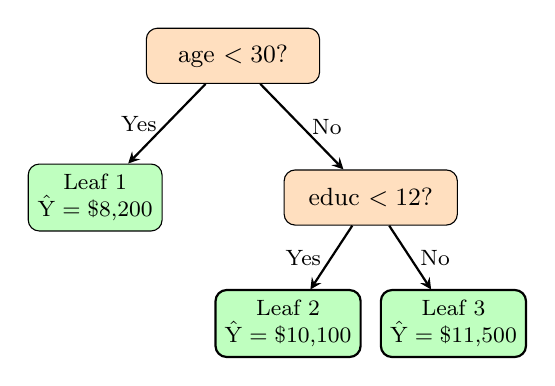
\begin{tikzpicture}[
			level 1/.style={sibling distance=3.5cm, level distance=1.8cm},
			level 2/.style={sibling distance=2.1cm, level distance=1.6cm},
			internal/.style={draw, rounded corners, fill=orange!25,
				align=center, font=\small,
				minimum width=2.2cm, minimum height=0.7cm},
			leaf/.style={draw, rounded corners, fill=green!25,
				align=center, font=\footnotesize,
				minimum width=1.7cm, minimum height=0.85cm},
			edge from parent/.style={draw, -stealth, thick}
		]
		\node[internal] {age $< 30$?}
			child {node[leaf] {Leaf 1\\ $\hat{\mathrm{Y}}=\$8{,}200$}
				edge from parent node[left, draw=none, fill=none,
					font=\footnotesize] {Yes}
			}
			child {node[internal] {educ $< 12$?}
				child {node[leaf] {Leaf 2\\ $\hat{\mathrm{Y}}=\$10{,}100$}
					edge from parent node[left, draw=none, fill=none,
						font=\footnotesize] {Yes}
				}
				child {node[leaf] {Leaf 3\\ $\hat{\mathrm{Y}}=\$11{,}500$}
					edge from parent node[right, draw=none, fill=none,
						font=\footnotesize] {No}
				}
				edge from parent node[right, draw=none, fill=none,
					font=\footnotesize] {No}
			};
		\end{tikzpicture}
		\end{center}
	\end{column}
	\begin{column}{0.48\textwidth}
		\small
		\begin{itemize}
			\item \textbf{Internal nodes} (orange): decision rules on $X$
			\vspace{0.2cm}
			\item \textbf{Leaves} (green): prediction $\hat{\mathrm{Y}}$ = mean of $\mathrm{Y}_i$ in that region
			\vspace{0.3cm}
			\item \textbf{Prediction}: follow branches until reaching a leaf
			\vspace{0.3cm}
			\item \textit{Example}: age $= 35$, educ $= 14$\\[4pt]
			$\rightarrow$ age $\geq 30$, educ $\geq 12$\\[2pt]
			$\rightarrow$ \textbf{Leaf 3}: $\hat{\mathrm{Y}} = \$11{,}500$
		\end{itemize}
	\end{column}
\end{columns}
\end{frame}




\begin{frame}{Decision Trees: Partition of Feature Space}
\begin{columns}[T]
	\begin{column}{0.52\textwidth}
		\vspace{0.3cm}
		\begin{center}
		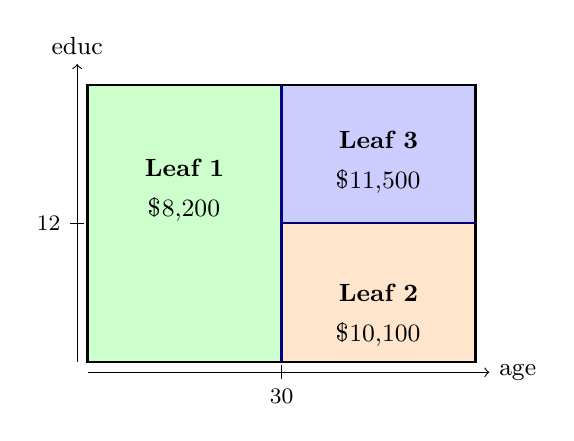
\begin{tikzpicture}[scale=0.88]
			% Fill regions first
			\fill[green!20]  (0,0) rectangle (2.8,4.0);
			\fill[orange!20] (2.8,0) rectangle (5.6,2.0);
			\fill[blue!20]   (2.8,2.0) rectangle (5.6,4.0);
			% Outer border
			\draw[thick] (0,0) rectangle (5.6,4.0);
			% Split 1: vertical at age=30
			\draw[thick, NavyBlue] (2.8,0) -- (2.8,4.0);
			% Split 2: horizontal at educ=12 (right half only)
			\draw[thick, NavyBlue] (2.8,2.0) -- (5.6,2.0);
			% Region labels
			\node[font={\small\bfseries}] at (1.4, 2.8) {Leaf 1};
			\node[font=\small] at (1.4, 2.2) {\$8,200};
			\node[font={\small\bfseries}] at (4.2, 1.0) {Leaf 2};
			\node[font=\small] at (4.2, 0.4) {\$10,100};
			\node[font={\small\bfseries}] at (4.2, 3.2) {Leaf 3};
			\node[font=\small] at (4.2, 2.6) {\$11,500};
			% Axes
			\draw[->] (0,-0.15) -- (5.8,-0.15) node[right, font=\small] {age};
			\draw[->] (-0.15,0) -- (-0.15,4.3) node[above, font=\small] {educ};
			% Axis ticks
			\draw (2.8,-0.05) -- (2.8,-0.25) node[below, font=\footnotesize] {30};
			\draw (-0.05,2.0) -- (-0.25,2.0) node[left, font=\footnotesize] {12};
		\end{tikzpicture}
		\end{center}
	\end{column}
	\begin{column}{0.48\textwidth}
		\small
		\begin{itemize}
			\item Each split divides the feature space into \textbf{rectangular regions}
			\vspace{0.3cm}
			\item All observations in the same region receive the \textbf{same prediction} (the in-region mean of $\mathrm{Y}$)
			\vspace{0.3cm}
			\item A \textbf{deeper tree} $\Rightarrow$ more splits $\Rightarrow$ smaller regions $\Rightarrow$ more flexible, but risks \textbf{overfitting}
			\vspace{0.3cm}
			\item The tree approximates any nonlinear relationship between $\mathrm{Y}$ and $X$ without specifying a functional form
		\end{itemize}
	\end{column}
\end{columns}
\end{frame}




%=============================================================
\title[]
{Random Forest}

\author{}
\institute{}
\date{}

\begin{frame}{}
	\titlepage
\end{frame}




\begin{frame}{Why a Single Decision Tree Is Not Enough}
	\begin{itemize}
		\item A single deep tree has a fundamental weakness: \textbf{high variance}
		\vspace{0.2cm}
		\begin{itemize}
			\item The tree ``memorizes'' the training data rather than learning the true pattern
			\vspace{0.2cm}
			\item Small changes in the data (e.g.\ adding or removing a few observations) can lead to a completely different tree structure
			\vspace{0.2cm}
			\item Predictions on new data are unstable and often poor
		\end{itemize}
		\vspace{0.2cm}
		\item \textbf{Intuition:} Like asking one person for an opinion --- noisy and unreliable
		\vspace{0.2cm}
		\item \textbf{Solution:} Ask many people independently and take the average
		\vspace{0.2cm}
		\begin{itemize}
			\item In ML: grow many diverse trees on different random subsamples and average their predictions
            		\vspace{0.2cm}
			\item This is \textbf{Random Forest} (Breiman, 2001)
		\end{itemize}
	\end{itemize}
\end{frame}





%-------------------------------------------------------------
%--- Page 1: data pattern ---
\begin{frame}{Why a Single Decision Tree Is Not Enough}{High Variance}
\begin{columns}[T]

\begin{column}{0.44\textwidth}
  \begin{center}\textbf{Sample A}\end{center}
  %\vspace{0.15cm}
  \begin{center}\small
  \begin{tabular}{@{}ccc@{}}
    \toprule
    Age & Educ & Wage \\
    \midrule
    20 & 12 & \$8  \\
    25 & 11 & \$9  \\
    40 & 12 & \$21 \\
    45 & 11 & \$22 \\
    50 & 12 & \$23 \\
    \bottomrule
  \end{tabular}
  \end{center}
 % \vspace{0.3cm}
  \begin{itemize}\small
    \item Age $<30$: wages \$8--9
          \vspace{0.1cm}

    \item Age $\geq30$: wages \$21--23
    %       \vspace{0.1cm}

    % \item Education: all 11--12, no variation
  \end{itemize}
      \vspace{0.1cm}
  $\Rightarrow$ \textbf{Tree splits on Age}
\end{column}
\hfill
\begin{column}{0.50\textwidth}
  \begin{center}\textbf{Sample B}\end{center}
 % \vspace{0.15cm}
  \begin{center}\small
  \begin{tabular}{@{}ccc@{}}
    \toprule
    Age & Educ & Wage \\
    \midrule
    20                   & 12                   & \$8                  \\
    \textcolor{red}{25}  & \textcolor{red}{16}  & \textcolor{red}{\$30}\\
    40                   & 12                   & \$21                 \\
    45                   & 11                   & \$22                 \\
    50                   & 12                   & \$23                 \\
    \bottomrule
  \end{tabular}
  \end{center}
  %\vspace{0.2cm}
  \begin{itemize}\small
    \item Age $<30$: \{\$8, \$30\} --- no longer predicts
      \vspace{0.1cm}
    \item Educ $=16\to\$30$; Educ $\leq12\to\$8$--23
  \end{itemize}
  \vspace{0.1cm}
  $\Rightarrow$ \textbf{Tree splits on Education}
\end{column}
\end{columns}
\end{frame}

%--- Page 2: RSS explanation ---
\begin{frame}{Why a Single Decision Tree Is Not Enough}{High Variance}

\textbf{Why does the tree change its split?}

\vspace{0.2cm}
\begin{center}
\begin{tabular}{@{}lcc@{}}
  \toprule
  Candidate split & RSS in Sample A & RSS in Sample B \\
  \midrule
  Age $< 30$  & \textbf{2.5} & 244 \\
  Educ $< 14$ & 217          & \textbf{149} \\
  \bottomrule
\end{tabular}
\end{center}

\vspace{0.2cm}
\begin{itemize}

\item The tree always picks the split with the lowest RSS:
\begin{itemize}
  \item Replacing 1 worker causes the RSS of the age split to explode: $2.5 \to 244$
  \vspace{0.1cm}
  \item The education split now has a lower RSS (149) $\Rightarrow$ tree switches to Education
  \vspace{0.1cm}
  \item[$\Rightarrow$] \textbf{High variance}: a tiny data change leads to a completely different tree
\end{itemize}
\end{itemize}

\end{frame}




%-------------------------------------------------------------
\begin{frame}{Why a Single Decision Tree Is Not Enough}{High Variance}
\begin{center}
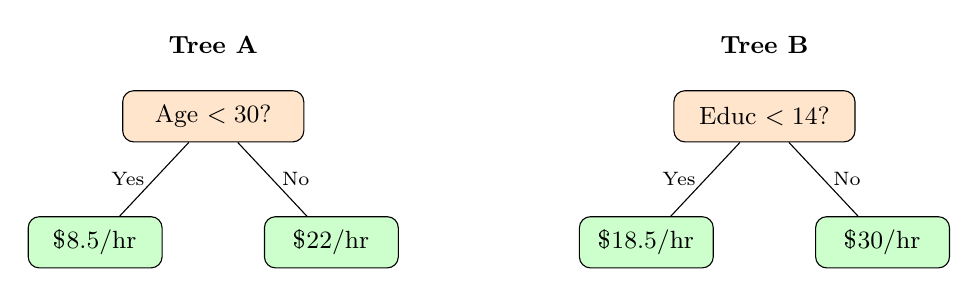
\begin{tikzpicture}[
  inode/.style={draw, rounded corners, fill=orange!20,
                align=center, font=\small,
                minimum width=2.3cm, minimum height=0.65cm},
  lnode/.style={draw, rounded corners, fill=green!20,
                align=center, font=\small,
                minimum width=1.7cm, minimum height=0.65cm},
  arr/.style={->, >=stealth, thick},
  level 1/.style={sibling distance=3.0cm, level distance=1.6cm},
  level 2/.style={sibling distance=1.9cm, level distance=1.5cm},
]
  %% ---- TREE A ----
  \begin{scope}[xshift=0.5cm]
    \node[font=\small, align=center] at (0,0.4)
      {\textbf{Tree A}};
    \node[inode] at (0,-0.5) {Age $< 30$?}
      child { node[lnode] {\$8.5/hr} edge from parent node[left,  font=\scriptsize]{Yes} }
      child { node[lnode] {\$22/hr}  edge from parent node[right, font=\scriptsize]{No}  };
  \end{scope}

  %% ---- VS label ----
  %\node[font=\large\bfseries, gray] at (5.5,-1.2) {vs.};

  %% ---- TREE B ----
  \begin{scope}[xshift=7.5cm]
    \node[font=\small, align=center] at (0,0.4)
      {\textbf{Tree B}};
    \node[inode] at (0,-0.5) {Educ $< 14$?}
      child { node[lnode] {\$18.5/hr} edge from parent node[left,  font=\scriptsize]{Yes} }
      child { node[lnode] {\$30/hr}   edge from parent node[right, font=\scriptsize]{No}  };
  \end{scope}
\end{tikzpicture}
\end{center}

\vspace{0.4cm}
\begin{itemize}
  \item Tree A splits on \textbf{Age}; Tree B splits on \textbf{Education} --- completely different logic
  \item Only \textbf{1 of the 5 workers} differs between the two samples
\end{itemize}
\end{frame}


%-------------------------------------------------------------
\begin{frame}{Why a Single Decision Tree Is Not Enough}{High Variance}

\begin{center}
  \textbf{New worker: Age = 22, Education = 16 years}\\[8pt]
  \small
  \begin{tabular}{@{}llc@{}}
    \toprule
     & Decision path & Predicted wage \\
    \midrule
    Tree A & Age $< 30$ $\to$ \textbf{Yes} & \$8.5/hr \\
    Tree B & Educ $< 14$ $\to$ \textbf{No} & \$30/hr \\
    \bottomrule
  \end{tabular}
\end{center}

\vspace{0.2cm}
\begin{itemize}
  \item Same worker, same features: yet predictions differ by \$21.5/hr
  \begin{itemize}

  \vspace{0.2cm}

  \item This is \textbf{high variance}: replacing just 1 training observation leads to wildly different predictions
  \vspace{0.2cm}

  \item \textbf{Solution}: average over many trees grown on different subsamples $\Rightarrow$ \textbf{Random Forest}
  \end{itemize}

\end{itemize}
\end{frame}




\begin{frame}{Random Forest: How It Works}{Algorithm}

\textbf{Two sources of randomness} ensure each tree is unique:
\vspace{0.2cm}
\begin{itemize}
  \item[\textbf{1.}] \textbf{Random subsampling}
  \begin{itemize}
    \vspace{0.1cm}
    \item Draw a random subset of observations and train each tree on it
    \vspace{0.1cm}
    \item Each tree sees different data $\Rightarrow$ learns a slightly different pattern
  \end{itemize}
  \vspace{0.25cm}
  \item[\textbf{2.}] \textbf{Random feature selection at each split}
  \begin{itemize}
    \vspace{0.1cm}
    \item At every candidate split, consider only $m$ randomly chosen covariates out of $p$ total
    \vspace{0.1cm}
    \item Typical choice: $m = \sqrt{p}$; \enspace e.g.\ 9 covariates $\Rightarrow$ consider only 3 at each split
    \vspace{0.1cm}
    \item Each tree uses different variables $\Rightarrow$ trees are diverse
  \end{itemize}
\end{itemize}

\vspace{0.35cm}
\textbf{Prediction for a new observation $x$:} average over all $B$ trees
\begin{equation*}
  \hat{Y}(x) \;=\; \frac{1}{B}\sum_{b=1}^{B} \hat{Y}_{b}(x)
\end{equation*}
\end{frame}




%-------------------------------------------------------------
\begin{frame}{Random Forest: How It Works}{Why Does Averaging Reduce Variance?}

\textbf{Intuition}: asking one person for an opinion is noisy; asking 100 people and averaging is far more reliable --- Random Forest does the same with trees

\vspace{0.3cm}
\begin{itemize}
  \item If $B$ independent trees each have variance $\sigma^2$, the average has variance
  \begin{equation*}
    \operatorname{Var}\!\left(\frac{1}{B}\sum_{b=1}^{B}\hat{Y}_{b}\right)
    = \frac{\sigma^2}{B} \;\xrightarrow{B\to\infty}\; 0
  \end{equation*}

  \item Trees trained on the same dataset are not fully independent, but the two sources of randomness keep correlation between trees low
  \vspace{0.1cm}
  \begin{itemize}
    \item Low correlation $\Rightarrow$ averaging still substantially reduces variance
  \end{itemize}
\end{itemize}

\vspace{0.3cm}
\begin{center}
\begin{tabular}{lccc}
  \toprule
                   & Bias & Variance       & Overfitting risk \\
  \midrule
  Single deep tree & Low  & \textbf{High}  & High \\
  Random Forest    & Low  & \textbf{Low}   & Low  \\
  \bottomrule
\end{tabular}
\end{center}
\end{frame}




\begin{frame}{Random Forest}{Illustration}
\begin{center}
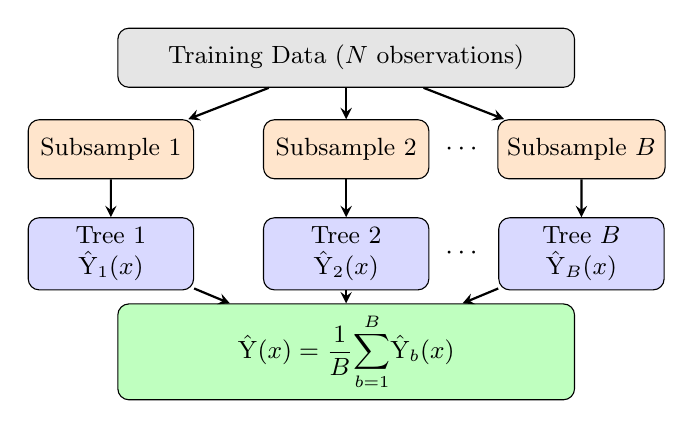
\begin{tikzpicture}[scale=0.83,
	box/.style={draw, rounded corners, minimum width=2.1cm, minimum height=0.75cm,
		align=center, font=\small},
	arr/.style={-stealth, thick}
]
	% Full dataset
	\node[box, fill=gray!20, minimum width=5.8cm] (data) at (0, 4.2)
		{Training Data ($N$ observations)};

	% Subsamples
	\node[box, fill=orange!20] (s1) at (-3.6, 2.8) {Subsample 1};
	\node[box, fill=orange!20] (s2) at (0,    2.8) {Subsample 2};
	\node[box, fill=orange!20] (s3) at (3.6,  2.8) {Subsample $B$};
	\node at (1.8, 2.8) {$\cdots$};

	\draw[arr] (data) -- (s1);
	\draw[arr] (data) -- (s2);
	\draw[arr] (data) -- (s3);

	% Trees
	\node[box, fill=blue!15] (t1) at (-3.6, 1.2)
		{Tree 1\\ $\hat{\mathrm{Y}}_1(x)$};
	\node[box, fill=blue!15] (t2) at (0,    1.2)
		{Tree 2\\ $\hat{\mathrm{Y}}_2(x)$};
	\node[box, fill=blue!15] (t3) at (3.6,  1.2)
		{Tree $B$\\ $\hat{\mathrm{Y}}_B(x)$};
	\node at (1.8, 1.2) {$\cdots$};

	\draw[arr] (s1) -- (t1);
	\draw[arr] (s2) -- (t2);
	\draw[arr] (s3) -- (t3);

	% Average prediction
	\node[box, fill=green!25, minimum width=5.8cm] (avg) at (0, -0.3)
		{$\hat{\mathrm{Y}}(x)=\dfrac{1}{B}{\displaystyle\sum_{b=1}^{B}}\hat{\mathrm{Y}}_{b}(x)$};

	\draw[arr] (t1) -- (avg);
	\draw[arr] (t2) -- (avg);
	\draw[arr] (t3) -- (avg);
\end{tikzpicture}
\end{center}
\vspace{-0.2cm}
\begin{itemize}
	\item Each tree is grown on a different subsample $\Rightarrow$ trees are diverse and their errors tend to cancel
\end{itemize}
\end{frame}











%=============================================================
\title[]
{Causal Tree}

\author{}
\institute{}
\date{}

\begin{frame}{}
	\titlepage
\end{frame}




\begin{frame}{From Prediction to Causal Inference}
	\begin{itemize}
		\item Random Forest predicts \textbf{outcomes}: given a person's characteristics $X_i$, estimate their expected wage $\hat{Y}(x)$
		\vspace{0.3cm}
		\item In program evaluation we want to answer a different question:
		\vspace{0.2cm}
		\begin{itemize}
			\item \textbf{Who benefits most from job training?}
			\vspace{0.1cm}
			\item Does the effect depend on age, education, or prior experience?
			\vspace{0.1cm}
			\item This is the \textbf{CATE}: $\tau(x) = \mathrm{E}[Y^1_i - Y^0_i \mid X_i = x]$
		\end{itemize}
		\vspace{0.3cm}
		\item \textbf{Can we adapt the tree idea?}
		\vspace{0.2cm}
		\begin{itemize}
			\item Decision tree: splits to make \textbf{wages} most different across leaves\\
			$\quad\Rightarrow$ finds ``who earns more?''
			\vspace{0.15cm}
			\item \textbf{Causal tree}: splits to make \textbf{treatment effects} most different across leaves\\
			$\quad\Rightarrow$ finds ``who benefits more from training?''
		\end{itemize}
	\end{itemize}
\end{frame}




\begin{frame}{Causal Tree}{Main Idea}
	\begin{itemize}
		\item \textbf{Setup:} a job training program
		\vspace{0.15cm}
		\begin{itemize}
			\item \textbf{Treatment group} ($D_i = 1$): workers who received training
			\item \textbf{Control group} ($D_i = 0$): workers who did not receive training
			\item \textbf{Outcome} $Y_i$: wage after the program
		\end{itemize}
		\vspace{0.25cm}
		\item A \textbf{causal tree} partitions workers into subgroups (leaves) and \textbf{compares treated vs.\ control} within each leaf
		\vspace{0.25cm}
		\item \textbf{Algorithm (Recursive Binary Splitting):}
		\vspace{0.15cm}
		\begin{itemize}
			\item[1] Find the variable $X^j$ and split point $s$ that makes treatment effects \textbf{most different} across the two groups
			\vspace{0.15cm}
			\item[2] Divide workers into two groups: $\{X^j < s\}$ and $\{X^j \geq s\}$
			\vspace{0.15cm}
			\item[3] Repeat within each group until a stopping rule is met
		\end{itemize}
		\vspace{0.25cm}
		\item The estimate in each \textbf{leaf} $\ell$ is:
		\[
			\hat{\tau}(\ell) = \bar{Y}^{1}_\ell - \bar{Y}^{0}_\ell
			\quad \text{(treated mean} - \text{control mean)}
		\]
	\end{itemize}
\end{frame}




\begin{frame}{Causal Tree}{Finding the Best Split}
\textbf{How to find $(X^j,\, s)$ that maximises treatment effect heterogeneity:}
\vspace{0.25cm}
\begin{enumerate}
	\item For each variable $X^j$ and each candidate $s$, split workers into two groups:
	\[
		R_1(j,s) = \{i: X^j_i < s\}, \qquad R_2(j,s) = \{i: X^j_i \geq s\}
	\]

	\item In each group, compute the \textbf{treatment effect} (treated mean $-$ control mean):
	\[
		\hat{\tau}(R) = \bar{Y}^{1}_{R} - \bar{Y}^{0}_{R}
	\]

	\item Compute the \textbf{difference in treatment effects} across the two groups:
	\[
		\Delta(j,s) = |\hat{\tau}(R_1) - \hat{\tau}(R_2)|
	\]

	\item Choose the $(j^*, s^*)$ that gives the \textbf{largest} $\Delta$ and repeat recursively
\end{enumerate}
\end{frame}




\begin{frame}{Causal Tree}{Finding the Best Split: Example}
\textbf{Example:} 10 workers, treatment $=$ job training

\vspace{0.25cm}
\begin{center}
\small
\begin{tabular}{lp{2.5cm}p{2.5cm}c}
	\hline
	\textbf{Candidate split}
		& $\hat{\tau}(R_1)$ \newline treated$-$control
		& $\hat{\tau}(R_2)$ \newline treated$-$control
		& $\Delta$ \\
	\hline
	Age $< 30$   & \$2{,}500 & \$400   & \textbf{\$2{,}100} $\;\leftarrow$ selected \\
	Educ $< 12$  & \$800     & \$2{,}600 & \$1{,}800 \\
	\hline
\end{tabular}
\end{center}

\vspace{0.25cm}
\begin{itemize}
	\item \textbf{Age $< 30$ is selected}: the training effect for young workers (\$2,500) is far larger than for older workers (\$400)
	\vspace{0.2cm}
	\item In contrast, a Decision Tree would pick whichever split best \textit{predicts wages} --- an entirely different criterion
\end{itemize}
\end{frame}




\begin{frame}{Causal Tree}{The Bias Problem}
\begin{itemize}
	\item After finding the split that maximises $\Delta(j,s)$, we compute $\hat{\tau}(\ell) = \bar{Y}^1_\ell - \bar{Y}^0_\ell$ \textbf{using the same data}
	\vspace{0.2cm}
	\item This creates \textbf{adaptive bias}: the tree searched many possible splits and selected the one with the largest effect difference --- the estimates are inflated
	\vspace{0.2cm}
	\item Analogy: run 20 hypothesis tests and report only the most significant result --- the reported $p$-value is misleading
	\vspace{0.2cm}
	\item \textbf{Why necessary to fix?}
	\vspace{0.1cm}
	\begin{itemize}
		\item We cannot trust the leaf-level estimates $\hat{\tau}(\ell)$ for statistical inference
	\end{itemize}
\end{itemize}
\vspace{0.2cm}
\begin{center}
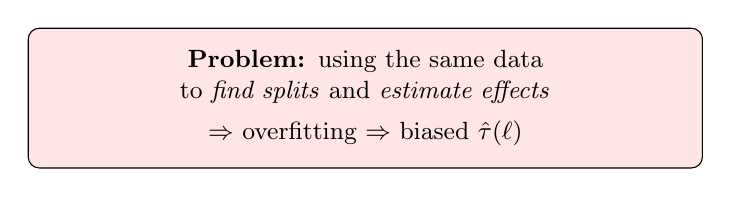
\begin{tikzpicture}
	\node[draw, rounded corners, fill=red!10, text width=8cm,
		align=center, font=\small, inner sep=8pt] {
		\textbf{Problem:} using the same data to \textit{find splits} and \textit{estimate effects}\\[4pt]
		$\Rightarrow$ overfitting $\Rightarrow$ biased $\hat{\tau}(\ell)$
	};
\end{tikzpicture}
\end{center}
\end{frame}




\begin{frame}{Honest Estimation}{Athey \& Imbens (2016)}
\begin{itemize}
	\item \textbf{Key idea:} Split the data into two halves, each with a \textit{different job}
	\vspace{0.3cm}
	\item \textbf{Step 1 --- Training sample $\mathcal{S}^{tr}$} \quad \textit{(find the tree structure)}
	\vspace{0.1cm}
	\begin{itemize}
		\item Search for splits that separate subgroups with different treatment effects
		\vspace{0.1cm}
		\item Decides: which variable to split on, and where
		\vspace{0.1cm}
		\item \textbf{Does not estimate any treatment effects}
	\end{itemize}
	\vspace{0.3cm}
	\item \textbf{Step 2 --- Estimation sample $\mathcal{S}^{est}$} \quad \textit{(measure effects in each leaf)}
	\vspace{0.1cm}
	\begin{itemize}
		\item Each worker is assigned to a leaf using the tree from Step 1
		\vspace{0.1cm}
		\item Within each leaf: $\hat{\tau}(\ell) = \bar{Y}^{1}_\ell - \bar{Y}^{0}_\ell$ \quad (treated minus control)
		\vspace{0.1cm}
		\item \textbf{$\mathcal{S}^{est}$ had no role in choosing splits $\Rightarrow$ no cherry-picking $\Rightarrow$ unbiased}
	\end{itemize}
\end{itemize}
\end{frame}




\begin{frame}{Honest Estimation}{Illustration}
\begin{center}
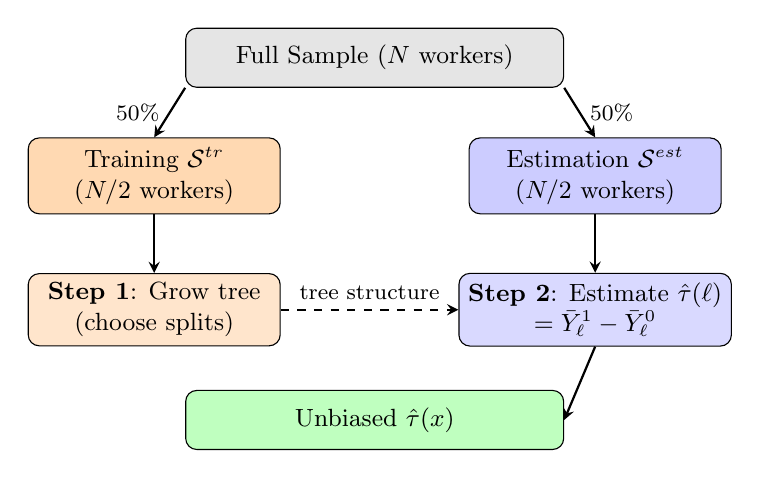
\begin{tikzpicture}[
	box/.style={draw, rounded corners, minimum width=3.2cm, minimum height=0.75cm,
		align=center, font=\small},
	arr/.style={-stealth, thick}
]
	\node[box, fill=gray!20, minimum width=4.8cm] (data) at (0, 4)
		{Full Sample ($N$ workers)};
	\node[box, fill=orange!30] (train) at (-2.8, 2.5)
		{Training $\mathcal{S}^{tr}$\\ ($N/2$ workers)};
	\node[box, fill=blue!20] (est) at (2.8, 2.5)
		{Estimation $\mathcal{S}^{est}$\\ ($N/2$ workers)};
	\draw[arr] (data.south west) -- (train.north)
		node[midway, left, font=\footnotesize] {50\%};
	\draw[arr] (data.south east) -- (est.north)
		node[midway, right, font=\footnotesize] {50\%};
	\node[box, fill=orange!20] (grow) at (-2.8, 0.8)
		{\textbf{Step 1}: Grow tree\\ (choose splits)};
	\draw[arr] (train) -- (grow);
	\node[box, fill=blue!15] (leaf) at (2.8, 0.8)
		{\textbf{Step 2}: Estimate $\hat{\tau}(\ell)$\\ $= \bar{Y}^1_\ell - \bar{Y}^0_\ell$};
	\draw[arr] (est) -- (leaf);
	\draw[arr, dashed] (grow.east) -- (leaf.west)
		node[midway, above, font=\footnotesize] {tree structure};
	\node[box, fill=green!25, minimum width=4.8cm] (out) at (0, -0.6)
		{Unbiased $\hat{\tau}(x)$};
	\draw[arr] (leaf.south) -- (out.east);
\end{tikzpicture}
\end{center}
\vspace{-0.1cm}
\begin{itemize}
	\item Splitting the data eliminates \textbf{adaptive bias}: the tree cannot overfit to the same workers used to estimate effects
\end{itemize}
\end{frame}




\begin{frame}{Causal Tree: Illustration}
\begin{columns}[T]
	\begin{column}{0.52\textwidth}
	\begin{center}
	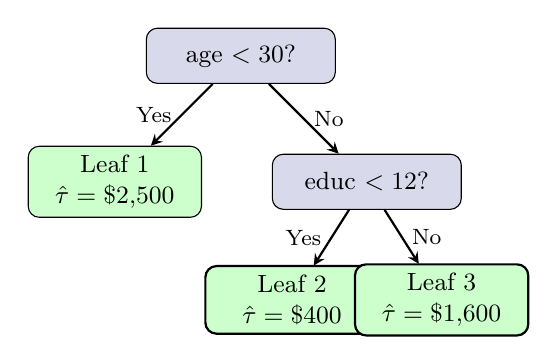
\begin{tikzpicture}[
		internal/.style={draw, rounded corners, fill=NavyBlue!15,
			minimum width=2.4cm, minimum height=0.7cm, align=center, font=\small},
		leaf/.style={draw, rounded corners, fill=green!20,
			minimum width=2.2cm, minimum height=0.85cm, align=center, font=\small},
		edge from parent/.style={draw, -stealth, thick},
		level 1/.style={sibling distance=3.2cm, level distance=1.6cm},
		level 2/.style={sibling distance=1.9cm, level distance=1.5cm}
	]
		\node[internal] {age $< 30$?}
			child {node[leaf] {Leaf 1\\ $\hat{\tau}=\$2{,}500$}
				edge from parent node[left, draw=none, fill=none,
					font=\footnotesize] {Yes}}
			child {node[internal] {educ $< 12$?}
				child {node[leaf] {Leaf 2\\ $\hat{\tau}=\$400$}
					edge from parent node[left, draw=none, fill=none,
						font=\footnotesize] {Yes}}
				child {node[leaf] {Leaf 3\\ $\hat{\tau}=\$1{,}600$}
					edge from parent node[right, draw=none, fill=none,
						font=\footnotesize] {No}}
				edge from parent node[right, draw=none, fill=none,
					font=\footnotesize] {No}};
	\end{tikzpicture}
	\end{center}
	\end{column}
	\begin{column}{0.48\textwidth}
	\small
	\begin{itemize}
		\item \textbf{Internal nodes}: splitting rules on $X$
		\vspace{0.2cm}
		\item \textbf{Leaves}: $\hat{\tau}(\ell) = \bar{Y}^1_\ell - \bar{Y}^0_\ell$
		\vspace{0.3cm}
		\item \textbf{Prediction}: follow branches until reaching a leaf
		\vspace{0.3cm}
		\item \textit{Example}: worker with age $= 35$, educ $= 9$\\[4pt]
		$\rightarrow$ age $\geq 30$, educ $< 12$\\[2pt]
		$\rightarrow$ \textbf{Leaf 2}: $\hat{\tau} = \$400$
	\end{itemize}
	\end{column}
\end{columns}
\end{frame}




\begin{frame}{Causal Tree: Partition of Feature Space}
\begin{columns}[T]
	\begin{column}{0.52\textwidth}
	\vspace{0.2cm}
	\begin{center}
	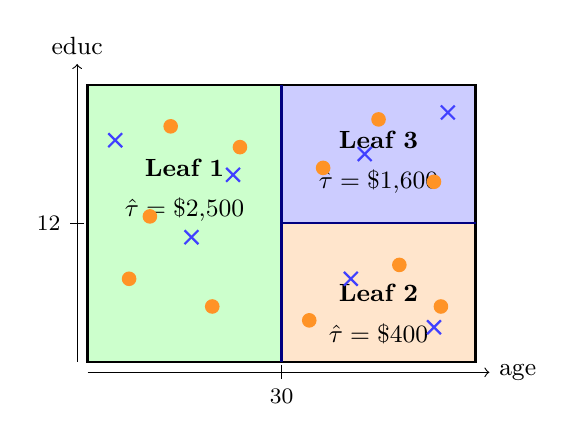
\begin{tikzpicture}[scale=0.88]
		% Fill regions
		\fill[green!20]  (0,0) rectangle (2.8,4.0);
		\fill[orange!20] (2.8,0) rectangle (5.6,2.0);
		\fill[blue!20]   (2.8,2.0) rectangle (5.6,4.0);
		% Outer border
		\draw[thick] (0,0) rectangle (5.6,4.0);
		% Split lines
		\draw[thick, NavyBlue] (2.8,0) -- (2.8,4.0);
		\draw[thick, NavyBlue] (2.8,2.0) -- (5.6,2.0);
		% Region labels
		\node[font={\small\bfseries}] at (1.4, 2.8) {Leaf 1};
		\node[font=\small] at (1.4, 2.2) {$\hat{\tau}=\$2{,}500$};
		\node[font={\small\bfseries}] at (4.2, 1.0) {Leaf 2};
		\node[font=\small] at (4.2, 0.4) {$\hat{\tau}=\$400$};
		\node[font={\small\bfseries}] at (4.2, 3.2) {Leaf 3};
		\node[font=\small] at (4.2, 2.6) {$\hat{\tau}=\$1{,}600$};
		% Treated dots
		\foreach \x/\y in {0.6/1.2, 1.2/3.4, 0.9/2.1, 1.8/0.8, 2.2/3.1}
			\fill[orange!85] (\x,\y) circle (3pt);
		% Control crosses
		\foreach \x/\y in {0.4/3.2, 1.5/1.8, 2.1/2.7} {
			\draw[blue!75, thick] (\x-0.1,\y-0.1)--(\x+0.1,\y+0.1);
			\draw[blue!75, thick] (\x+0.1,\y-0.1)--(\x-0.1,\y+0.1);
		}
		\foreach \x/\y in {3.2/0.6, 4.5/1.4, 5.1/0.8}
			\fill[orange!85] (\x,\y) circle (3pt);
		\foreach \x/\y in {3.8/1.2, 5.0/0.5} {
			\draw[blue!75, thick] (\x-0.1,\y-0.1)--(\x+0.1,\y+0.1);
			\draw[blue!75, thick] (\x+0.1,\y-0.1)--(\x-0.1,\y+0.1);
		}
		\foreach \x/\y in {3.4/2.8, 4.2/3.5, 5.0/2.6}
			\fill[orange!85] (\x,\y) circle (3pt);
		\foreach \x/\y in {4.0/3.0, 5.2/3.6} {
			\draw[blue!75, thick] (\x-0.1,\y-0.1)--(\x+0.1,\y+0.1);
			\draw[blue!75, thick] (\x+0.1,\y-0.1)--(\x-0.1,\y+0.1);
		}
		% Axes
		\draw[->] (0,-0.15) -- (5.8,-0.15) node[right, font=\small] {age};
		\draw[->] (-0.15,0) -- (-0.15,4.3) node[above, font=\small] {educ};
		\draw (2.8,-0.05) -- (2.8,-0.25) node[below, font=\footnotesize] {30};
		\draw (-0.05,2.0) -- (-0.25,2.0) node[left, font=\footnotesize] {12};
	\end{tikzpicture}
	\end{center}
	\end{column}
	\begin{column}{0.48\textwidth}
	\small
	\begin{itemize}
		\item Each split divides the feature space into \textbf{rectangular regions}
		\vspace{0.25cm}
		\item {\color{orange!85!black}$\bullet$} = treated ($D_i=1$),\quad {\color{blue!75}$\times$} = control ($D_i=0$)
		\vspace{0.25cm}
		\item In each region: $\hat{\tau}(\ell) = \bar{Y}^1_\ell - \bar{Y}^0_\ell$
		\vspace{0.25cm}
		\item CIA: workers in the same leaf have similar $X$ $\Rightarrow$ treated and control are comparable $\Rightarrow$ \textbf{local experiment}
		\vspace{0.25cm}
		\item A \textbf{deeper tree} $\Rightarrow$ smaller regions, but fewer treated/control per leaf $\Rightarrow$ noisier $\hat{\tau}$
	\end{itemize}
	\end{column}
\end{columns}
\end{frame}




\begin{frame}{From Causal Tree to Causal Forest}
\begin{itemize}
	\item A single honest causal tree solves the \textbf{bias} problem --- but still has \textbf{high variance}
	\vspace{0.15cm}
	\begin{itemize}
		\item Small data changes can alter the tree structure substantially
		\item Each leaf contains few observations $\Rightarrow$ noisy estimates of $\hat{\tau}(\ell)$
	\end{itemize}
	\vspace{0.2cm}
	\item \textbf{Solution:} the same fix as Random Forest --- grow many trees and average
	\vspace{0.1cm}
	\begin{itemize}
		\item[$\Rightarrow$] \textbf{Causal Forest} (Wager \& Athey, 2018): $B$ honest causal trees on random subsamples
	\end{itemize}
\end{itemize}
\vspace{0.1cm}
\begin{center}
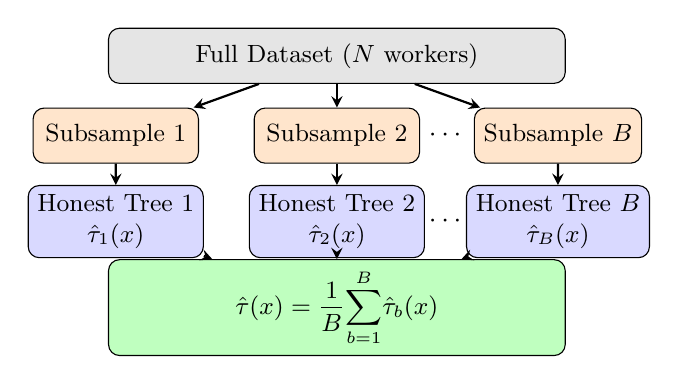
\begin{tikzpicture}[scale=0.78,
	box/.style={draw, rounded corners, minimum width=2.1cm, minimum height=0.7cm,
		align=center, font=\small},
	arr/.style={-stealth, thick}
]
	\node[box, fill=gray!20, minimum width=5.8cm] (data) at (0, 3.6)
		{Full Dataset ($N$ workers)};
	\node[box, fill=orange!20] (s1) at (-3.6, 2.3) {Subsample 1};
	\node[box, fill=orange!20] (s2) at (0, 2.3) {Subsample 2};
	\node[box, fill=orange!20] (s3) at (3.6, 2.3) {Subsample $B$};
	\node at (1.8, 2.3) {$\cdots$};
	\draw[arr] (data) -- (s1);
	\draw[arr] (data) -- (s2);
	\draw[arr] (data) -- (s3);
	\node[box, fill=blue!15] (t1) at (-3.6, 0.9) {Honest Tree 1\\ $\hat{\tau}_1(x)$};
	\node[box, fill=blue!15] (t2) at (0, 0.9) {Honest Tree 2\\ $\hat{\tau}_2(x)$};
	\node[box, fill=blue!15] (t3) at (3.6, 0.9) {Honest Tree $B$\\ $\hat{\tau}_B(x)$};
	\node at (1.8, 0.9) {$\cdots$};
	\draw[arr] (s1) -- (t1);
	\draw[arr] (s2) -- (t2);
	\draw[arr] (s3) -- (t3);
	\node[box, fill=green!25, minimum width=5.8cm] (avg) at (0, -0.5)
		{$\hat{\tau}(x)=\dfrac{1}{B}{\displaystyle\sum_{b=1}^{B}}\hat{\tau}_{b}(x)$};
	\draw[arr] (t1) -- (avg);
	\draw[arr] (t2) -- (avg);
	\draw[arr] (t3) -- (avg);
\end{tikzpicture}
\end{center}
\end{frame}









%=============================================================
\title[]
{Causal Forest}

\author{}
\institute{}
\date{}

\begin{frame}{}
	\titlepage
\end{frame}




\begin{frame}{Causal Forest}{Algorithm}
\textbf{Same principle as Random Forest, applied to treatment effect estimation:}
\vspace{0.25cm}
\begin{enumerate}
	\item Draw a random subsample of workers from the full dataset
	\vspace{0.2cm}
	\item Grow one \textbf{honest causal tree} on the subsample:
	\vspace{0.1cm}
	\begin{itemize}
		\item \textbf{Training half:} find splits that maximise $|\hat{\tau}(R_1) - \hat{\tau}(R_2)|$
		\item \textbf{Estimation half:} compute $\hat{\tau}(\ell) = \bar{Y}^1_\ell - \bar{Y}^0_\ell$ in each leaf
	\end{itemize}
	\vspace{0.2cm}
	\item Repeat $B$ times (e.g., $B = 2{,}000$ trees)
	\vspace{0.2cm}
	\item For each worker $i$, average all tree estimates:
	\[
		\hat{\tau}(x_i) = \frac{1}{B}\sum_{b=1}^{B} \hat{\tau}_b(x_i)
	\]
\end{enumerate}
\end{frame}




\begin{frame}{Causal Forest}{Why Averaging Reduces Variance}
\begin{itemize}
	\item A single honest causal tree has \textbf{high variance}: changing a few observations can produce a completely different tree structure
	\vspace{0.3cm}
	\item Each tree makes a noisy estimate of $\tau(x)$:
	\[
		\hat{\tau}_b(x) = \tau(x) + \varepsilon_b
	\]
	\vspace{0.1cm}
	where $\varepsilon_b$ is estimation noise specific to subsample $b$
	\vspace{0.3cm}
	\item Because each tree uses a \textbf{different random subsample}, the errors $\varepsilon_b$ are approximately independent across trees
	\vspace{0.3cm}
	\item Averaging cancels out the noise:
	\[
		\frac{1}{B}\sum_{b=1}^{B}\hat{\tau}_b(x)
		\;=\; \tau(x) + \underbrace{\frac{1}{B}\sum_{b=1}^{B}\varepsilon_b}_{\;\to\, 0 \text{ as } B \to \infty}
	\]
\end{itemize}
\end{frame}




\begin{frame}{Causal Forest}{Statistical Properties}
\begin{itemize}
	\item \textbf{Consistency:} as the sample size grows, the estimates converge to the true effects
	\[
		\hat{\tau}(x) \;\xrightarrow{\;p\;}\; \tau(x) \quad \text{as } N \to \infty
	\]
	\vspace{0.1cm}
	\item \textbf{Asymptotic normality:} each individual estimate $\hat{\tau}(x_i)$ is approximately normally distributed
	\vspace{0.3cm}
	\item[$\Rightarrow$] We can construct valid \textbf{confidence intervals} for each worker's treatment effect
	\vspace{0.3cm}
	\item \textbf{Why this matters:} unlike a standard Random Forest, a Causal Forest supports \textbf{statistical inference} --- we can test whether the treatment effect is significantly positive for a given subgroup
\end{itemize}
\end{frame}




\begin{frame}{Causal Forest}{Causal Forest vs.\ Random Forest}
\begin{center}
\begin{tabular}{lcc}
	\hline
	& \textbf{Random Forest} & \textbf{Causal Forest} \\
	\hline
	\textbf{Goal}      & predict $\hat{Y}(x)$  & estimate $\hat{\tau}(x)$ \\[4pt]
	\textbf{Split}     & minimise RSS($Y$)     & maximise $|\hat{\tau}(R_1) - \hat{\tau}(R_2)|$ \\[4pt]
	\textbf{Leaf est.} & $\bar{Y}_\ell$        & $\bar{Y}^1_\ell - \bar{Y}^0_\ell$ \\[4pt]
	\textbf{Data req.} & outcome $Y$, covariates $X$ & also needs treatment $D$ \\[4pt]
	\textbf{Honest}    & no                    & yes (split/estimation samples) \\[4pt]
	\textbf{Inference} & no                    & yes (confidence intervals) \\
	\hline
\end{tabular}
\end{center}
\vspace{0.3cm}
\begin{itemize}
	\item The two methods share the same tree-and-forest machinery; the key difference is the \textbf{objective}: predicting $Y$ vs.\ estimating the causal effect of $D$ on $Y$
\end{itemize}
\end{frame}




\begin{frame}{Causal Forest}{Individual CATE Estimates}
\begin{itemize}
	\item After estimation, each worker $i$ receives a \textbf{personalised} estimate $\hat{\tau}(x_i)$
	\vspace{0.2cm}
	\item \textbf{Interpretation:} $\hat{\tau}(x_i)$ is the estimated wage gain from job training for a worker with characteristics $x_i$
\end{itemize}
\vspace{0.2cm}
\textbf{Example:}
\vspace{0.1cm}
\begin{center}
\small
\begin{tabular}{lcccc}
	\hline
	& Age & Educ & Leaf ($\bar{Y}^1 - \bar{Y}^0$) & $\hat{\tau}(x_i)$ \\
	\hline
	Worker A & 24 & 10 & \$9,800 $-$ \$7,300 & \$2,500 \\
	Worker B & 42 & 11 & \$11,200 $-$ \$10,800 & \$400 \\
	Worker C & 38 & 14 & \$12,100 $-$ \$10,500 & \$1,600 \\
	\hline
\end{tabular}
\end{center}
\vspace{0.2cm}
\begin{itemize}
	\item \textbf{Heterogeneity:} training benefits young workers (\$2,500) much more than older workers (\$400)
	\vspace{0.1cm}
	\item These estimates guide \textbf{policy targeting}: who should be prioritised for training?
\end{itemize}
\end{frame}




\begin{frame}{After Estimating CATE}{Average Treatment Effect (ATE)}
\begin{itemize}
	\item The causal forest produces an individual estimate $\hat{\tau}(x_i)$ for every worker
	\vspace{0.3cm}
	\item \textbf{Average Treatment Effect:} aggregate all individual estimates into one number
	\[
		\hat{\tau}^{ATE} = \frac{1}{N}\sum_{i=1}^{N}\hat{\tau}(x_i)
	\]
	\vspace{0.1cm}
	\item \textbf{Interpretation:} the average wage gain from job training across all workers in the sample
	\vspace{0.3cm}
	\item \textbf{Key features:}
	\vspace{0.1cm}
	\begin{itemize}
		\item Comparable to ATE estimated by OLS or IV
		\vspace{0.15cm}
		\item Comes with a valid standard error $\Rightarrow$ can test $H_0: \tau^{ATE} = 0$
		\vspace{0.15cm}
		\item Can also compute \textbf{ATT} (average effect on the treated): average only over $D_i = 1$
	\end{itemize}
\end{itemize}
\end{frame}




\begin{frame}{After Estimating CATE}{Distribution of Treatment Effects}
\begin{itemize}
	\item Plot a \textbf{histogram} of all individual CATE estimates $\hat{\tau}(x_i)$
	\vspace{0.3cm}
	\item \textbf{Reading the histogram:}
	\vspace{0.1cm}
	\begin{itemize}
		\item The \textbf{mean} of the distribution = ATE
		\vspace{0.15cm}
		\item \textbf{Wide spread} $\Rightarrow$ large heterogeneity: job training helps some workers much more than others --- targeting matters
		\vspace{0.15cm}
		\item \textbf{Narrow spread} $\Rightarrow$ homogeneous effects: most workers benefit about the same amount
	\end{itemize}
	\vspace{0.3cm}
	\item \textbf{Policy implication:} if the distribution is wide, it is worthwhile to identify \textit{who} benefits most and target the programme accordingly
\end{itemize}
\end{frame}




\begin{frame}{After Estimating CATE}{Best Linear Projection (BLP)}
\begin{itemize}
	\item \textbf{Question:} which worker characteristics are associated with larger training effects?
	\vspace{0.3cm}
	\item \textbf{Method:} regress the estimated CATE $\hat{\tau}(x_i)$ on covariates $X_i$:
	\[
		\hat{\tau}(x_i) = \beta_0 + \beta_1\,\text{age}_i + \beta_2\,\text{educ}_i + \beta_3\,\text{re74}_i + \cdots + \varepsilon_i
	\]
	\vspace{0.15cm}
	\item \textbf{Interpretation:}
	\vspace{0.1cm}
	\begin{itemize}
		\item $\hat{\beta}_1 < 0$: older workers tend to benefit \textit{less} from training
		\vspace{0.1cm}
		\item $\hat{\beta}_3 < 0$: workers with higher prior earnings benefit less
	\end{itemize}
	\vspace{0.3cm}
	\item \textbf{Key advantage:} valid standard errors allow testing $H_0: \beta_j = 0$
	\vspace{0.1cm}
	\begin{itemize}
		\item Does characteristic $j$ \textit{significantly} predict treatment benefit?
	\end{itemize}
\end{itemize}
\end{frame}




\begin{frame}{After Estimating CATE}{Variable Importance}
\begin{itemize}
	\item \textbf{Question:} which covariates most consistently drive the splits across all $B$ trees?
	\vspace{0.3cm}
	\item \textbf{Method:} for each variable $X^j$, count how often it is used for splitting across all trees (weighted by split depth)
	\vspace{0.3cm}
	\item \textbf{Interpretation:} a high-importance variable is one the forest repeatedly identifies as creating the most treatment effect heterogeneity
	\vspace{0.3cm}
	\item \textbf{Distinction from BLP:}
	\vspace{0.1cm}
	\begin{itemize}
		\item BLP: linear regression of $\hat{\tau}(x_i)$ on $X_i$ --- gives coefficients with standard errors
		\vspace{0.1cm}
		\item Variable importance: non-parametric measure --- captures nonlinear and interaction effects without assuming a functional form
	\end{itemize}
	\vspace{0.2cm}
	\item Both tools together answer: \textit{``who benefits, and why?''}
\end{itemize}
\end{frame}




%=============================================================
\title[]
{R Example: Job Training Program}

\author{}
\institute{}
\date{}

\begin{frame}{}
	\titlepage
\end{frame}




\begin{frame}{R Example: LaLonde (1986) Job Training Data}{Overview}
	LaLonde, Robert J. (1986), ``\textbf{Evaluating the Econometric Evaluations of Training Programs with Experimental Data}'', \textit{American Economic Review}

	\vspace{0.2cm}
	\begin{itemize}
		\item A classic randomized experiment on the effect of job training on earnings
		\vspace{0.2cm}
		\begin{itemize}
			\item \textbf{Treatment $D_i$:} Participation in job training (National Supported Work Demonstration)
			\vspace{0.2cm}
			\item \textbf{Outcome $Y_i$:} Earnings in 1978 (re78)
		\end{itemize}
		\vspace{0.2cm}
		\item Covariates $X_i$: age, years of education, race (Black, Hispanic), marital status, no high school degree, pre-treatment earnings (1974, 1975)
		\vspace{0.2cm}
		\item Sample: $n = 445$ individuals (185 treated, 260 control)
		\vspace{0.2cm}
		\item \textbf{Question:} The average effect of training is well-established. \textbf{Who benefits most?}
	\end{itemize}
\end{frame}




\begin{frame}[fragile]{R Example: Job Training Program}{Data and Code}
	\begin{itemize}
		\item See \textbf{CausalForest.R}
		\vspace{0.2cm}
		\item Use the LaLonde dataset from the \textbf{Matching} package
		\vspace{0.2cm}
		\item Install the following packages:
		\begin{itemize}
			\vspace{0.2cm}
			\item \textbf{grf}: Generalized Random Forests (causal forest)
			\vspace{0.2cm}
			\item \textbf{Matching}: contains the LaLonde dataset
			\vspace{0.2cm}
			\item \textbf{ggplot2}: visualization
		\end{itemize}
	\end{itemize}
\end{frame}




\begin{frame}[fragile]{R Example: Job Training Program}{Install Packages}
\begin{lstlisting}[language=R]
install.packages(c("grf", "Matching", "ggplot2"))

library(grf)
library(Matching)
library(ggplot2)
\end{lstlisting}
	\begin{itemize}
		\item \textbf{grf}: Main package for causal forest estimation
		\vspace{0.2cm}
		\item \textbf{Matching}: Provides the LaLonde dataset
		\vspace{0.2cm}
		\item \textbf{ggplot2}: For visualizing CATE distribution
	\end{itemize}
\end{frame}




\begin{frame}[fragile]{R Example: Job Training Program}{Load and Prepare Data}
\begin{lstlisting}[language=R]
data(lalonde)

# Define outcome, treatment, and covariates
Y <- lalonde$re78
D <- lalonde$treat
X <- lalonde[, c("age", "educ", "black", "hisp",
                 "married", "nodegree", "re74", "re75")]
X <- as.matrix(X)
\end{lstlisting}
	\begin{itemize}
		\item \textbf{Y}: Earnings in 1978 (outcome variable)
		\vspace{0.2cm}
		\item \textbf{D}: Binary treatment indicator (1 = received job training)
		\vspace{0.2cm}
		\item \textbf{X}: Matrix of pre-treatment covariates
	\end{itemize}
\end{frame}




\begin{frame}[fragile]{R Example: Job Training Program}{Estimate Causal Forest}
\begin{lstlisting}[language=R]
# Set seed for reproducibility
set.seed(2025)

# Estimate causal forest
cf <- causal_forest(X = X, Y = Y, W = D,
                    num.trees = 2000)
\end{lstlisting}
	\begin{itemize}
		\item \textbf{causal\_forest()}: Estimates a causal forest
		\vspace{0.2cm}
		\begin{itemize}
			\item \textbf{X}: Covariate matrix
			\vspace{0.2cm}
			\item \textbf{Y}: Outcome variable
			\vspace{0.2cm}
			\item \textbf{W}: Binary treatment variable
			\vspace{0.2cm}
			\item \textbf{num.trees}: Number of trees in the forest (default: 2000)
		\end{itemize}
		\vspace{0.2cm}
		\item The function automatically performs honest estimation using subsampling
	\end{itemize}
\end{frame}




\begin{frame}[fragile]{R Example: Job Training Program}{Average Treatment Effect}
\begin{lstlisting}[language=R]
# Estimate Average Treatment Effect (ATE)
ate <- average_treatment_effect(cf, target.sample = "all")
print(ate)
\end{lstlisting}
	\begin{itemize}
		\item \textbf{average\_treatment\_effect()}: Computes ATE from the causal forest
		\vspace{0.2cm}
		\begin{itemize}
			\item Returns estimate and standard error
			\vspace{0.2cm}
			\item \textbf{target.sample = "all"}: Average over all observations
		\end{itemize}
		\vspace{0.3cm}
		\item Can also estimate the \textbf{ATT} (Average Treatment effect on the Treated):
\begin{lstlisting}[language=R]
att <- average_treatment_effect(cf,
         target.sample = "treated")
\end{lstlisting}
	\end{itemize}
\end{frame}




\begin{frame}[fragile]{R Example: Job Training Program}{Individual CATE Estimates}
\begin{lstlisting}[language=R]
# Get CATE estimates for each individual
tau_hat <- predict(cf)$predictions

# Summary statistics
summary(tau_hat)
\end{lstlisting}
	\begin{itemize}
		\item \textbf{predict(cf)}: Returns a data frame with individual CATE estimates $\hat{\tau}(x_i)$
		\vspace{0.2cm}
		\item Each individual receives a personalized treatment effect estimate
		\vspace{0.3cm}
		\item We can examine:
		\vspace{0.2cm}
		\begin{itemize}
			\item The distribution of CATE across individuals
			\vspace{0.2cm}
			\item Which individuals have the largest (or smallest) treatment effects
		\end{itemize}
	\end{itemize}
\end{frame}




\begin{frame}[fragile]{R Example: Job Training Program}{Visualize CATE Distribution}
\begin{lstlisting}[language=R]
cate_df <- data.frame(tau_hat = tau_hat)

ggplot(cate_df, aes(x = tau_hat)) +
  geom_histogram(bins = 30, fill = "steelblue",
                 color = "white") +
  geom_vline(xintercept = mean(tau_hat),
             color = "red", linetype = "dashed") +
  labs(title = "Distribution of CATE Estimates",
       x = "Estimated Treatment Effect",
       y = "Count") +
  theme(plot.background = element_rect(fill = "white"))
\end{lstlisting}
	\begin{itemize}
		\item The red dashed line marks the \textbf{average} treatment effect
		\vspace{0.2cm}
		\item Spread of the histogram shows the degree of \textbf{heterogeneity}
	\end{itemize}
\end{frame}




\begin{frame}[fragile]{R Example: Job Training Program}{Best Linear Projection}
\begin{lstlisting}[language=R]
# Best Linear Projection of CATE on covariates
blp <- best_linear_projection(cf, X)
print(blp)
\end{lstlisting}
	\begin{itemize}
		\item \textbf{best\_linear\_projection()}: Regresses estimated CATE on covariates
		\vspace{0.3cm}
		\item Interprets output:
		\vspace{0.2cm}
		\begin{itemize}
			\item \textbf{educ}: Does education increase or decrease the training effect?
			\vspace{0.2cm}
			\item \textbf{re74, re75}: Do workers with lower pre-treatment earnings benefit more?
			\vspace{0.2cm}
			\item \textbf{nodegree}: Do workers without a high school degree benefit more?
		\end{itemize}
		\vspace{0.3cm}
		\item Coefficients have valid standard errors for statistical inference
	\end{itemize}
\end{frame}




\begin{frame}[fragile]{R Example: Job Training Program}{Variable Importance}
\begin{lstlisting}[language=R]
# Variable importance
var_imp <- variable_importance(cf)
names(var_imp) <- colnames(X)

# Sort and plot
var_imp_df <- data.frame(variable = names(var_imp),
                          importance = var_imp)
var_imp_df <- var_imp_df[order(-var_imp_df$importance), ]
print(var_imp_df)
\end{lstlisting}
	\begin{itemize}
		\item Shows which covariates are most frequently used for splitting across trees
		\vspace{0.2cm}
		\item Identifies the key drivers of treatment effect heterogeneity
	\end{itemize}
\end{frame}




\begin{frame}[fragile]{R Example: Job Training Program}{CATE vs. Covariates}
\begin{lstlisting}[language=R]
# Plot CATE against education
plot_df <- data.frame(educ = lalonde$educ,
                      tau_hat = tau_hat)

ggplot(plot_df, aes(x = educ, y = tau_hat)) +
  geom_point(alpha = 0.5) +
  geom_smooth(method = "loess", se = TRUE,
              color = "blue") +
  labs(title = "CATE by Years of Education",
       x = "Years of Education",
       y = "Estimated Treatment Effect") +
  theme(plot.background = element_rect(fill = "white"))
\end{lstlisting}
	\begin{itemize}
		\item Plots individual CATE estimates against education
		\vspace{0.2cm}
		\item Reveals how the job training effect varies with education level
	\end{itemize}
\end{frame}



%-------------------------------------------------------------
\begin{frame}[fragile]{R Example: Exporting Results to Stata}{Workflow for Post-Analysis}
\begin{columns}[T]
\begin{column}{0.48\textwidth}
\textbf{Step 1: Export from R}
\vspace{0.15cm}

\begin{lstlisting}[language=R]
# Export CATE estimates to CSV
results <- data.frame(
  id      = 1:nrow(X),
  tau_hat = tau_hat,
  age     = lalonde$age,
  educ    = lalonde$educ,
  treat   = lalonde$treat
)
write.csv(results,
  "cate_results.csv",
  row.names = FALSE)
\end{lstlisting}
\end{column}
\hfill
\begin{column}{0.48\textwidth}
\textbf{Step 2: Analyse in Stata}
\vspace{0.15cm}

\begin{lstlisting}[language=Stata]
* Import CATE estimates
import delimited ///
  "cate_results.csv", clear

* Distribution of CATE
histogram tau_hat, ///
  normal kdensity ///
  xtitle("Estimated CATE")

* BLP: Best Linear Predictor
* (Chernozhukov et al. 2018)
reg tau_hat age educ, robust
\end{lstlisting}
\end{column}
\end{columns}
\vspace{0.2cm}
\begin{itemize}
  \item \textbf{Stata has no native causal forest package} — all forest estimation must be done in R (\texttt{grf})
  \item Export \texttt{tau\_hat} to CSV/DTA, then use Stata for familiar post-analysis (BLP regression, histograms, subgroup summaries)
\end{itemize}
\end{frame}




%=============================================================
\title[]
{Labor Economics Application}

\author{}
\institute{}
\date{}

\begin{frame}{}
	\titlepage
\end{frame}




\begin{frame}{Labor Economics Applications of Causal Forest}
	\begin{itemize}
		\item Causal Forest has been applied to several important labor economics questions:
		\vspace{0.3cm}
		\item[] Knaus, Michael C., Michael Lechner, and Anthony Strittmatter (2021), ``\textbf{Heterogeneous Employment Effects of Job Search Programmes}'', \textit{Journal of Labor Economics}
		\vspace{0.2cm}
		\begin{itemize}
			\item Uses causal forest to identify subgroups who benefit most from job search assistance programs
			\vspace{0.2cm}
			\item Finds that workers with lower labor market attachment benefit more
		\end{itemize}
		\vspace{0.3cm}
		\item[] Davis, Jonathan M.V. and Sara B. Heller (2020), ``\textbf{Rethinking the Benefits of Youth Employment Programs}'', \textit{NBER Working Paper}
		\vspace{0.2cm}
		\begin{itemize}
			\item Applies causal forest to a randomized summer youth employment program
			\vspace{0.2cm}
			\item Identifies which at-risk youth benefit most in terms of reduced violence
		\end{itemize}
	\end{itemize}
\end{frame}




\begin{frame}{Why Causal Forest Matters for Labor Economics Policy}
	\begin{itemize}
		\item \textbf{Policy targeting:} Identify which workers should be prioritized for job training, unemployment benefits, or active labor market programs
		\vspace{0.3cm}
		\item \textbf{Minimum wage:} Do employment effects differ by firm size, region, or worker skill?
		\vspace{0.3cm}
		\item \textbf{Education returns:} Does the return to college vary by family background, field of study, or local labor market?
		\vspace{0.3cm}
		\item \textbf{Parental leave:} Do effects on maternal labor supply differ by pre-birth earnings, industry, or marital status?
		\vspace{0.3cm}
		\item \textbf{Key insight:} A policy with a small or zero \textbf{average} effect may still have large positive effects for a specific subgroup
		\vspace{0.2cm}
		\begin{itemize}
			\item Causal forest helps us find and characterize that subgroup
		\end{itemize}
	\end{itemize}
\end{frame}




%=============================================================
\title[]
{Recommended Resources}

\author{}
\institute{}
\date{}

\begin{frame}{}
	\titlepage
\end{frame}




\begin{frame}{Recommended Resources for Self-Learning}
	\begin{itemize}
		\item Machine Learning \& Causal Inference: A Short Course (Stanford)
		\vspace{0.2cm}
		\begin{itemize}
			\item \url{https://www.gsb.stanford.edu/faculty-research/centers-initiatives/sil/research/methods/ai-machine-learning/short-course}
			\vspace{0.2cm}
		\end{itemize}
		\item \textbf{grf} package documentation and vignettes
		\vspace{0.2cm}
		\begin{itemize}
			\item \url{https://grf-labs.github.io/grf/}
			\vspace{0.2cm}
		\end{itemize}
		\item Susan Athey and Stefan Wager's course materials on ML and causal inference
		\vspace{0.2cm}
		\begin{itemize}
			\item \url{https://github.com/susanathey/causalForest}
		\end{itemize}
	\end{itemize}
\end{frame}




\begin{frame}{Recommended Resources for Self-Learning}
	\begin{itemize}
		\item One free textbook: \textit{An Introduction to Statistical Learning} (James et al.)
		\vspace{0.2cm}
		\begin{itemize}
			\item Website: \url{https://www.statlearning.com/}
			\vspace{0.2cm}
			\item Covers decision trees and random forests in detail (Chapter 8)
		\end{itemize}
		\vspace{0.3cm}
		\item NBER Summer Institute 2013: Econometric Methods for High-Dimensional Data
		\vspace{0.2cm}
		\begin{itemize}
			\item \url{https://www.nber.org/econometrics_minicourse_2013/}
		\end{itemize}
		\vspace{0.3cm}
		\item Athey \& Imbens (2019), ``\textbf{Machine Learning Methods That Economists Should Know About}'', \textit{Annual Review of Economics}
		\vspace{0.2cm}
		\begin{itemize}
			\item Accessible overview of ML for causal inference
		\end{itemize}
	\end{itemize}
\end{frame}


\end{document}
